%% equivalent_genome_features.tex
%% Author: Leighton Pritchard
%% Copyright: James Hutton Institute
%% A brief description of genome feature prediction, and related
%% issues

% SUBSECTION: Genome Features
\subsection{What makes genome features equivalent?}

% What do you align, and why?
\begin{frame}
  \frametitle{What makes genome features equivalent?}
  \begin{center}
    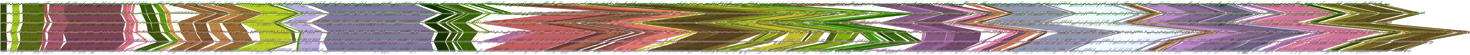
\includegraphics[width=1\textwidth]{images/collinear_zeae}  
  \end{center}
  When we compare two features (e.g. genes) between two or more genomes, there must be some basis for making the comparison \\
  That is, they have to be \textit{equivalent} in some way, such as:
  \begin{itemize}
    \item common evolutionary origin
    \item functional similarity
    \item a family-based relationship
  \end{itemize}
  It's common to define equivalence of genome features in terms of evolutionary relationship.
\end{frame}

% Gene features
\begin{frame}
  \frametitle{Evolutionary relationships\footnote{\tiny{Fitch (1970) \textit{Syst. Zool.} \textbf{19}:99-113 \href{http://dx.doi.org/10.2307/2412448}{doi:10.2307/2412448}}}}
  Equivalencies and relationships can be quite complex. \\
  We need precise terms to describe relationships between genome features. \\
  \begin{center}
    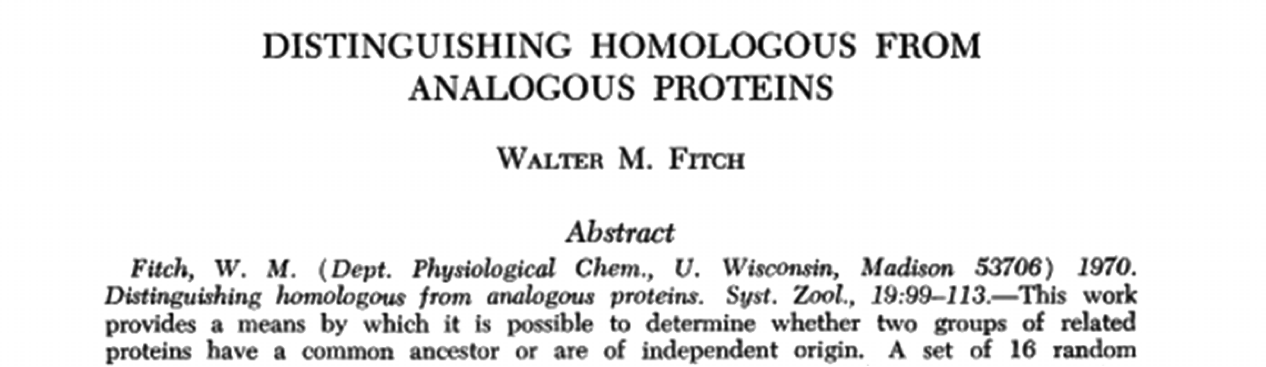
\includegraphics[width=1\textwidth]{images/fitch}  
  \end{center}  
  \begin{itemize}
    \item \textbf{analogy}: functional similarity
    \item \textbf{homology}: evolutionary common ancestor
  \end{itemize}    
\end{frame}

